\chapter{Meltdown e il sistema di protezione KAISER}
La sicurezza dei sistemi informatici attuali si fonda sull'isolamento della memoria,
ad esempio marcando come privilegiati gli indirizzi di memoria kernel e bloccando eventuali
accessi da parte di programmi utente \cite{lettieri:protezione}. 
\textbf{Meltdown} è un tipo di attacco informatico che sfrutta un effetto
collaterale dell'esecuzione fuori ordine nei processori moderni per leggere locazioni di memoria scelte in maniera
arbitraria. L'attacco funziona su varie microarchitetture Intel prodotte sin dal 2010, indipendentemente dal sistema
operativo in uso. Meltdown è quindi in grado di accedere arbitrariamente a qualsiasi locazione di memoria protetta
(afferenti al kernel o ad altri processi) senza necessitare alcun permesso o privilegio da parte del
sistema \cite{lipp:meltdown}.

Meltdown rompe quindi tutti i meccanismi di sicurezza che si basano sull'isolamento degli spazi di indirizzamento, andando a colpire milioni di utenti. Il sistema di protezione KAISER, sviluppato originariamente per KASLR \cite{gruss:kaslr}, ha l'importante effetto secondario di impedire l'utilizzo di Meltdown \cite{lipp:meltdown}.


\section{Background}

\subsection[]{Esecuzione Fuori Ordine}
\label{sec:esecuzione-fuori-ordine}

\subsection{Spazi di indirizzamento}
\begin{figure}
	\centering
	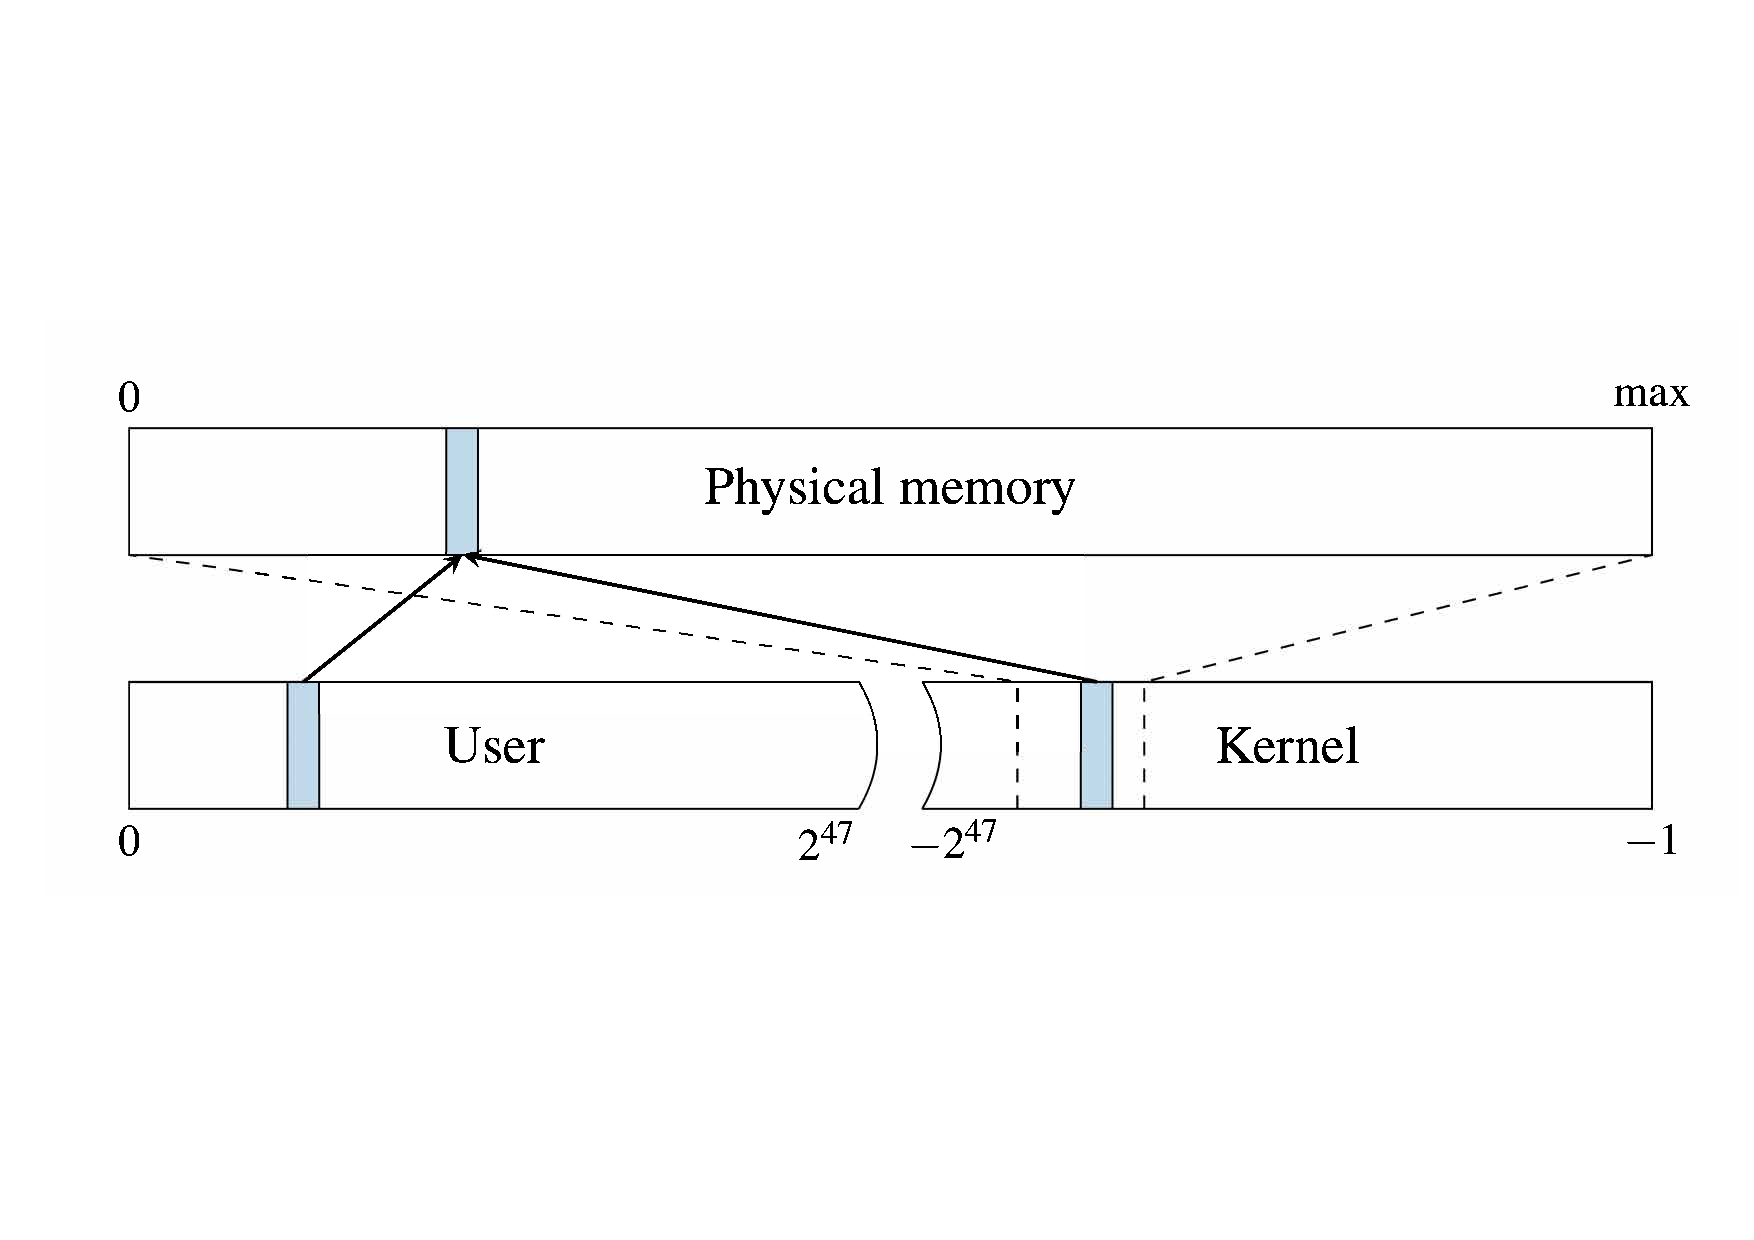
\includegraphics[width=0.5\textwidth]{"img/memoria-fisica.pdf"}
	\caption{text} % TODO
	\label{fig:memoria-fisica}
\end{figure}

Per risolvere diversi problemi, in particolare l'isolamento dei processi \cite{lettieri:paginazione}, le CPU supportano l'utilizzo di spazi d'indirizzamento virtuali, in cui gli indirizzi virtuali (relativi al singolo processo) vengono tradotti in indirizzi fisici. 
Lo spazio d'indirizzamento di un processo (ovvero tutti i possibili indirizzi che un processo può generare) viene suddiviso in regioni dette \emph{pagine} che possono essere mappate individualmente nella memoria fisica attraverso una tabella di traduzione multivello. 
Ogni processo possiede una propria tabella di traduzione che traduce tutti e soli i suoi indirizzi virtuali e che definisce le proprietà di protezione delle varie zone di memoria. 

Ogni processo può quindi riferirsi esclusivamente agli indirizzi appartenenti al proprio spazio di indirizzamento virtuale. Per permettere l'utilizzo 


\subsection{Attacchi Cache}
Al fine di velocizzare gli accessi alla RAM, le CPU contengono buffer di memoria molto veloce ma di dimensioni limitate che costituiscono la cosiddetta \emph{memoria cache}. La memoria cache maschera i tempi di latenza estremamente lunghi per l'accesso alla memoria centrale (molto lenta in confronto alla cache) conservando le locazioni di memoria che, secondo principi statistici come la \emph{località spaziale} (se un programma accede ad un certo indirizzo, è molto probabile che in breve tempo accederà ad un indirizzo vicino)  e la \emph{località temporale} (se un programma accede ad un certo indirizzo, è molto probabile che in breve tempo vi accederà di nuovo), è più probabile vengano indirizzate dalla CPU nel breve periodo \cite{lettieri:cache}.

Gli attacchi a canale laterale (\emph{side-channel attacks}) contro la cache sfruttano questa differenza di tempo di accesso introdotta dalla cache stessa. Negli attacchi Flush+Reload \cite{yaron:flush-reload}, usati da Meltdown \cite{lipp:meltdown}, l'attaccante è in grado di determinare se una locazione di memoria è stata precedentemente caricata in cache, misurando il tempo impiegato da un'operazione di lettura.

%%
\section{Come agisce Meltdown}
L'attacco Meltdown consiste in due fasi fondamentali \cite{lipp:meltdown}:
\begin{enumerate}
	\item Far eseguire alla CPU una o più istruzioni in maniera speculativa (le \emph{transient instruction}) che accedono a locazioni di memoria protetta (kernel o altri processi).
	\item Leggere gli effetti dell'esecuzione delle transient instruction a livello di microarchitettura per ottenere il contenuto delle locazioni di memoria accedute.
\end{enumerate}

\subsection{L'esecuzione delle transient instruction}
Nella prima fase di Meltdown, l'attaccante cerca di accedere ad una zona di memoria protetta, ad esempio la memoria kernel.
Il tentativo di accesso ad una pagina non accessibile da livello utente fa in modo che la CPU sollevi un'eccezione di protezione, che generalmente termina il processo. 
Tuttavia, a causa dell'esecuzione fuori ordine, la CPU potrebbe aver già eseguito l'istruzione di accesso in maniera speculativa prima delle istruzioni relative all'eccezione di protezione, al fine di minimizzare i tempi di latenza (vedi paragrafo \ref{sec:esecuzione-fuori-ordine}). 
Nonostan
